\documentclass[tikz, margin=0.1cm]{standalone}

\usepackage{stix2}

\begin{document}
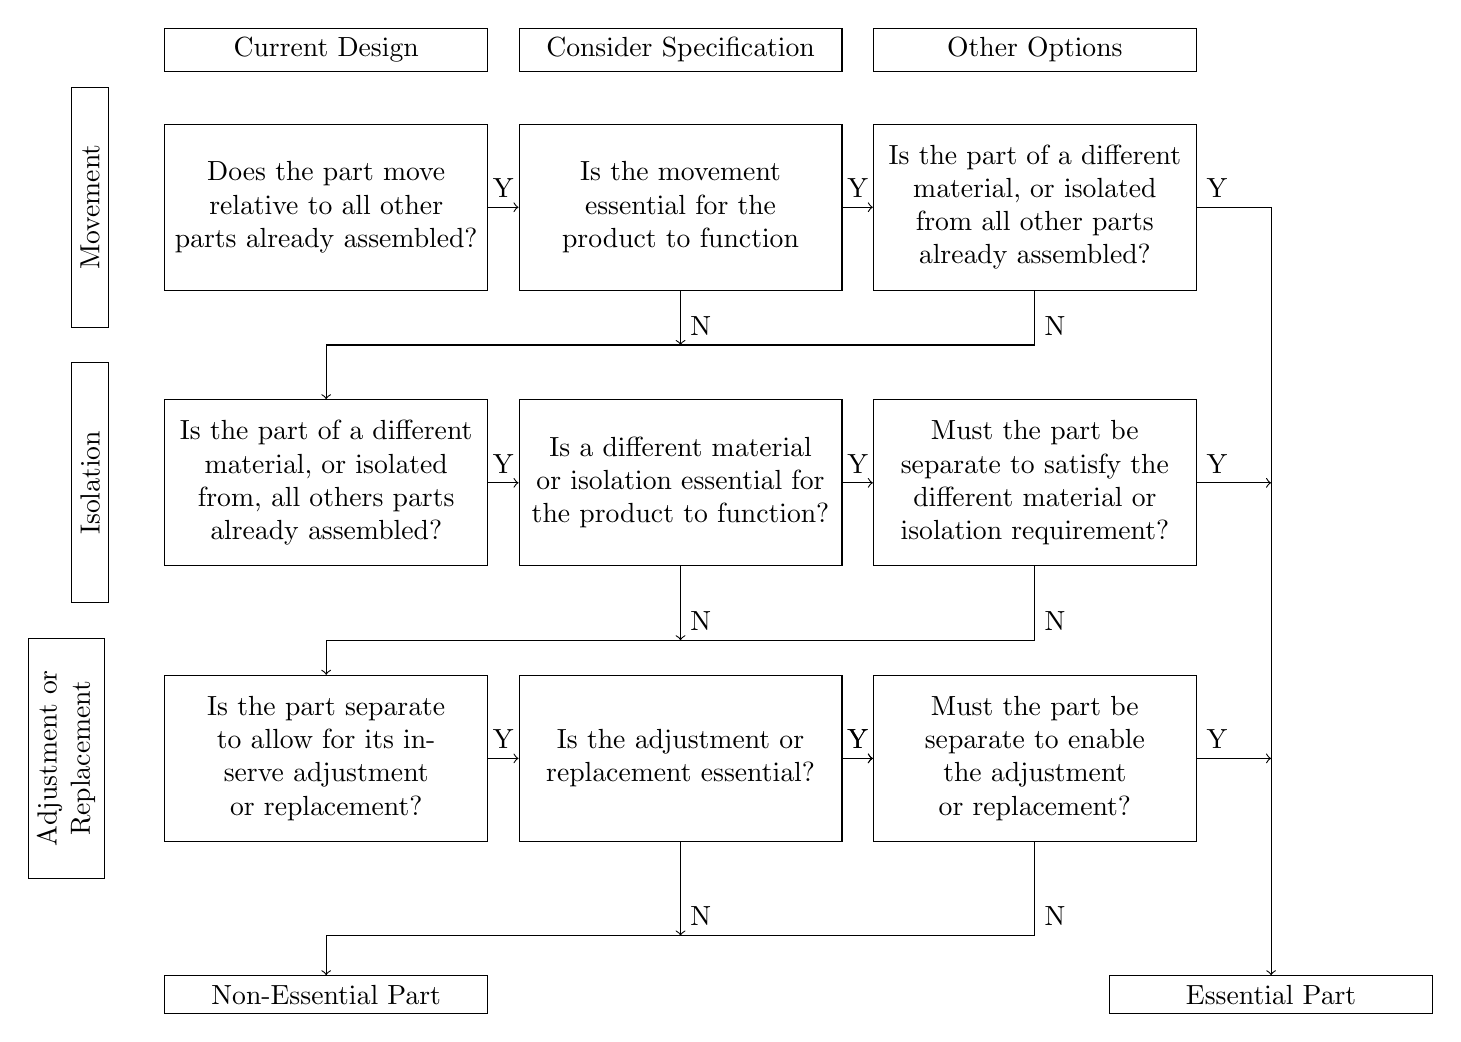
\begin{tikzpicture}%[scale=0.75, every node/.style={scale=0.75}]
    \node[align=center, draw, text width=110] at (0,0) {Current Design};
    
    \node[align=center, draw, text width=110] at (4.5,0) {Consider Specification};
    
    \node[align=center, draw, text width=110] at (9,0) {Other Options};
    
    \node[align=center, draw, text width=80, rotate=90] at (-3,-2) {Movement};
    
    \node[align=center, draw, text width=80, rotate=90] at (-3,-5.5) {Isolation};
    
    \node[align=center, draw, text width=80, rotate=90] at (-3.3,-9) {Adjustment or Replacement};
    
    \node[align=center, draw, text width=110, minimum height=60] (A) at (0,-2) {Does the part move relative to all other parts already assembled?};
    
    \node[align=center, draw, text width=110, minimum height=60] (B) at (4.5,-2) {Is the movement essential for the product to function};
    
    \node[align=center, draw, text width=110, minimum height=60] (C) at (9,-2) {Is the part of a different material, or isolated from all other parts already assembled?};
    
    \node[align=center, draw, text width=110, minimum height=60] (D) at (0,-5.5) {Is the part of a different material, or isolated from, all others parts already assembled?};
    
    \node[align=center, draw, text width=110, minimum height=60] (E) at (4.5,-5.5) {Is a different material or isolation essential for the product to function?};
    
    \node[align=center, draw, text width=110, minimum height=60] (F) at (9,-5.5) {Must the part be separate to satisfy the different material or isolation requirement?};
    
    \node[align=center, draw, text width=110, minimum height=60] (G) at (0,-9) {Is the part separate to allow for its in-serve adjustment or replacement?};
    
    \node[align=center, draw, text width=110, minimum height=60] (H) at (4.5,-9) {Is the adjustment or replacement essential?};
    
    \node[align=center, draw, text width=110, minimum height=60] (I) at (9,-9) {Must the part be separate to enable the adjustment or replacement?};
    
    \node[align=center, draw, text width=110] (J) at (0,-12) {Non-Essential Part};
    
    \node[align=center, draw, text width=110] (K) at (12,-12) {Essential Part};
    
    \draw[->] (A) -- (B) node[pos=0.5, anchor=south] {Y};
    \draw[->] (B) -- (C) node[pos=0.5, anchor=south] {Y};
    
    \draw[->] (D) -- (E) node[pos=0.5, anchor=south] {Y};
    \draw[->] (E) -- (F) node[pos=0.5, anchor=south] {Y};
    
    \draw[->] (G) -- (H) node[pos=0.5, anchor=south] {Y};
    \draw[->] (H) -- (I) node[pos=0.5, anchor=south] {Y};
    
    \draw[->] (H) -- (I) node[pos=0.5, anchor=south] {Y};
    
    \draw[->] (C) -- (9,-3.75) -| (D) node[pos=0, anchor=south west] {N};
    \draw[->] (B) -- (4.5,-3.75) node[pos=1, anchor=south west] {N};
    
    \draw[->] (F) -- (9,-7.5) -| (G) node[pos=0, anchor=south west] {N};
    \draw[->] (E) -- (4.5,-7.5) node[pos=1, anchor=south west] {N};
    
    \draw[->] (I) -- (9,-11.25) -| (J) node[pos=0, anchor=south west] {N};
    \draw[->] (H) -- (4.5,-11.25) node[pos=1, anchor=south west] {N};
    
    \draw[->] (C) -| (K) node[pos=0, anchor=south west] {Y};
    \draw[->] (F) -- (12,-5.5) node[pos=0, anchor=south west] {Y};
    \draw[->] (I) -- (12,-9) node[pos=0, anchor=south west] {Y};

\end{tikzpicture}
\end{document}